\documentclass[12pt,hidelinks]{article}

\usepackage[margin=1in]{geometry}
\usepackage{amsmath}
\usepackage{graphicx}
\usepackage{cclicenses}
\usepackage{fancyhdr,lastpage}
\usepackage[]{hyperref}
\pagestyle{fancy}
\usepackage{enumitem}
\setlist{nosep}
\setlist[enumerate]{label=(\alph*)}
\usepackage{tcolorbox}
\usepackage{fancyvrb}
\VerbatimFootnotes
\usepackage{tikz}
\usepackage{siunitx}

\renewcommand{\thesection}{\Roman{section}.}

\lhead{TUTORIAL: NEWTON'S LAWS: DEALING WITH AIR RESISTANCE}
\rhead{}
\lfoot{Tutorial 3, Week 5 \\\cc 2024 East Carolina University}
\cfoot{}
\rfoot{{\bf Page \thepage \hspace*{0.4em}of \pageref{LastPage}}\\Contact: \url{wolfs15@ecu.edu}}

\newcommand{\checkin}{{\bf \noindent $\Rightarrow$ PAUSE and check with an instructor or another
  group.}} 

\begin{document}


\section{Air Resistance and Newton's Second Law}
Suppose that you took a small rubber ball to the top of a very tall building and dropped it
from rest at $t=0$. At a later time $t=t_a$, the ball moves with \textit{constant speed}. (The
constant speed eventually reached by the falling ball is called the \textit{terminal speed}.)
\begin{enumerate}
  \item In the space provided below, draw separate free-body diagrams for the ball (i) at
  $t=0$, and (ii) at $t=t_a$.  Clearly label all forces. \vfill

  What can be said about the acceleration of the ball (i) at $t=0$? (ii) at $t=t_a$? Discuss
  both magnitude and direction.  Explain how you can use your free-body diagrams above to
  support your answers. \vfill
  \item In the space below, sketch a qualitatively correct graph of velocity vs.\ time ($v$
  vs.\ $t$) for the ball.  On your graph, clearly label the instant $t=t_a$ on the horizontal
  axis.
  \begin{center}
    \begin{tikzpicture}[>=stealth]
      \draw[<->] (-1,0) -- (10,0) node [right]{$t$};
      \draw[<->] (0,-1) -- (0,5) node [left]{$v$};
    \end{tikzpicture}
  \end{center}
  On the same set of axes above, show the $v$ vs.\ $t$ graph that \textit{would have been}
  correct if there were \textit{no} air resistance.  Make sure your graph is consistent with
  your first $v$ vs.\ $t$ graph.  Describe in words how you made sure that both $v$ vs.\ $t$
  graphs were consistent with each other. \vfill
  \newpage
  \item Now imagine releasing the rubber ball at shoulder level so that the ball drops to the
  floor and bounces back straight up. Suppose that the upward speed of the ball immediately
  after it leaves the floor were \textit{exactly equal} to its downward speed immediately
  before it reaches the floor.  (Assume the ball never reaches terminal speed, but continue to
  take air resistance into account.)
  \begin{center}
    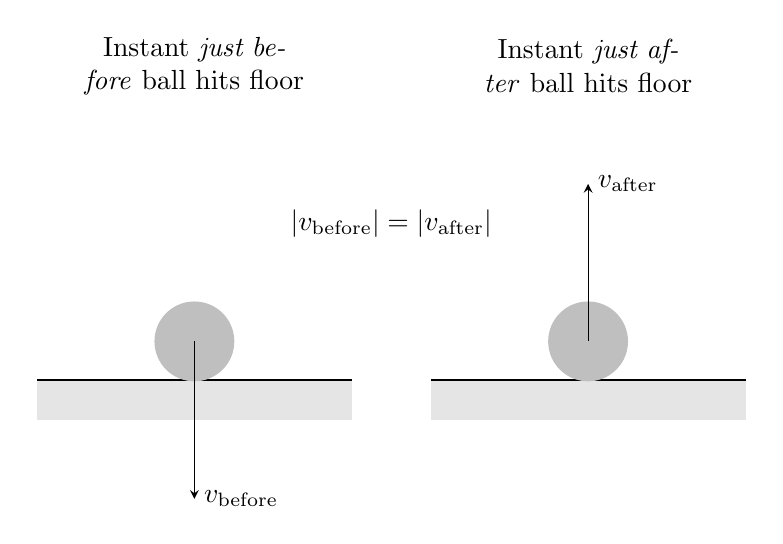
\begin{tikzpicture}[>=stealth]
      \draw[very thick] (0,0) -- (4,0);
      \fill[black!10!white] (0,-0.5) rectangle (4,0);
      \draw[very thick] (5,0) -- (9,0);
      \fill[black!10!white] (5,-0.5) rectangle (9,0);
      \filldraw[black!25!white] (2,0.5) circle (0.5);
      \draw[->] (2,0.5) -- (2,-1.5) node [right]{$v_{\text{before}}$};
      \filldraw[black!25!white] (7,0.5) circle (0.5);
      \draw[->] (7,0.5) -- (7,2.5) node [right]{$v_{\text{after}}$};
      \node[align=center, text width=4cm] at (2,4) {Instant \textit{just before} ball hits floor};
      \node[align=center, text width=4cm] at (7,4) {Instant \textit{just after} ball hits
        floor};
      \node[align=center] at (4.5,2) {$\left|v_{\text{before}}\right| = \left|v_{\text{after}}\right|$};
    \end{tikzpicture}
  \end{center}
  \begin{enumerate}[label=\arabic*.]
    \item Consider the following conversation between two students:
    \begin{description}
      \item[Student 1] ``Acceleration is derived from velocity, which is equal in magnitude at
      both instants.  That means that the ball has the same acceleration at both times.''
      \item[Student 2] ``That's right. In fact, if the ball has the same speed at both
      instants, then the force of air resistance is the same as well, so the net force is the
      same at both instants.''
    \end{description}
    In the space below, write down whether you \textit{agree} or \textit{disagree} with each
    student. Be nitpicky! \vfill
    \item Draw separate free body diagrams for the ball (i) immediately before it reaches the
    ground and (ii) immediately after it leaves the ground.  Clearly label each force. \vfill

    On the basis of your results, at which instant is the acceleration of the ball
    \textit{larger} in magnitude: (i) just before it reaches the ground, (ii) just after it
    leaves the ground, or (iii) is it the same at both instants?  Explain your
    reasoning. \vfill
    \item Refer again to the two statements from part 1.  Do you agree or disagree with each
    statement?  If you disagree with any of the student statements, identify the
    \textit{specific} error in reasoning used by that student.  Discuss your reasoning with
    your partners. \vfill
  \end{enumerate}
\end{enumerate}

\newpage
For the remainder of these exercises, we will consider the motion of spherical objects that fall
vertically in air (or some other viscous fluid).  In such a case, the force of air resistance
is treated as being:
\begin{enumerate}[label=(\roman*)]
  \item proportional to the speed of the object (with magnitude $c_1\left|v\right|$),
  \item proportional to the square of the speed (with magnitude $c_2v^2$), or
  \item a combination of the above two terms (linear and quadratic).
\end{enumerate}
where $c_1$ and $c_2$ are positive constants.

\section{Calculating Terminal Speed}
In answering the following questions, let vertically downward be defined as the positive
direction.
\begin{enumerate}
  \item Suppose that a small ball were moving with downward velocity $v$ (that is, $v>0$).
  Starting with Newton's 2\textsuperscript{nd} Law, write an equation that includes the
  acceleration $a$ of the ball and all relevant force terms ($mg$, $c_1v$, and
  $c_2v^2$).  In particular, carefully decide the sign (whether ``+'' or ``-'' that belongs in
  front of each individual term.  Discuss your reasoning with your partners. \vfill
  \item How would your equation in part (a) be different if the ball were instead moving
  \textit{upward} (that is, if $v<0$)? Explain. \vfill

  \checkin
  \item If the force of air resistance exerted were purely \textit{quadratic} with respect to
  velocity ($c_1= 0, c_2\neq 0$), use the appropriate equation to express the terminal velocity
  $v_t$ of the object in terms of $c_2, m,$ and $g$. \vfill

  Check that your expression for $v_t$ has the correct units.  That is, determine the
  appropriate units for $c_2$ and confirm that your expression for $v_t$ indeed has the
  appropriate units for a speed. \vfill
\end{enumerate}

\end{document}
